% LATEX TEMPLATE 
% adapted from https://infinitedescent.xyz/latex/ by wade_

\documentclass[11pt]{article}

% Edit the following to change the title, author name and date
\title{Calc in 3d Notes}
\author{saffron\_}
\date{}

% Packages
\usepackage{amsmath}
\usepackage{amsfonts}
\usepackage{amssymb}
\usepackage{amsthm}
\usepackage{enumerate}
\usepackage{geometry}
\usepackage{graphicx}
\usepackage{hyperref}
\usepackage{multicol}
% \usepackage[colorlinks=true,linkcolor=magenta]{hyperref}

% Page setup
\setlength{\parskip}{10pt}
\setlength{\parindent}{0pt}
\geometry{
    paper={letterpaper}, % Change to 'a4paper' for A4 size
    marginratio={1:1},
    margin={1in}
}

% Theorem environments
\theoremstyle{definition}
\newtheorem{theorem}{Theorem}
\newtheorem{lemma}[theorem]{Lemma}
\newtheorem{corollary}[theorem]{Corollary}
\newtheorem{proposition}[theorem]{Proposition}
\newtheorem{definition}[theorem]{Definition}
\newtheorem{example}[theorem]{Example}

% Custom per each document
\newcommand{\addsection}[1]{\section*{#1}\addcontentsline{toc}{section}{#1}} % for adding \section*{} sections to \tableofcontents
\newcommand{\bb}[1]{\mathbb{#1}} % love of my life
% \newcommand{\floor}[1]{\left\lfloor #1 \right\rfloor}
% \newcommand{\ceil}[1]{\left\lceil #1 \right\rceil}
\newcommand{\col}[1]{\begin{minipage}{\columnwidth}#1\end{minipage}}
\newcommand{\magn}[1]{\left\lVert #1 \right\rVert}
\DeclareMathOperator{\proj}{proj}
\DeclareMathOperator{\comp}{comp}

\graphicspath{ {./media/} }

\begin{document}
\maketitle
\tableofcontents

%%%%%%%%%%%%%%%%%%%%%%%%%%%%
%% Start of document body %%
%%%%%%%%%%%%%%%%%%%%%%%%%%%%

\newpage
\addsection{Chapter 2: Vectors in Space}

\begin{multicols}{2}[Graphing]
  \col{
    \centering
    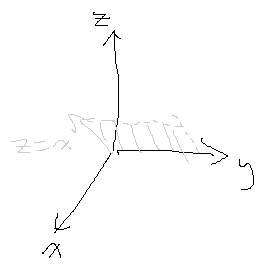
\includegraphics{3d_space.png}
    \emph{convention}
  }
  \col{
    \centering
    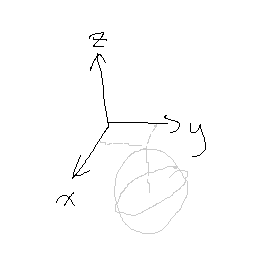
\includegraphics{sphere.png}
    \emph{sphere:} $(x-1)^2 + (y-2)^2 + (z+3)^2 = 9$
  }
\end{multicols}

\begin{multicols}{2}[The Vector]
  \col{
    \centering
    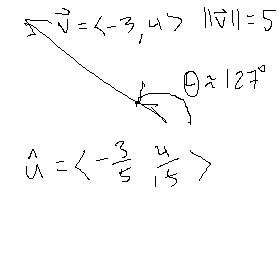
\includegraphics{vector.png}
  }
  \col{
    \begin{itemize}
      \item a quantity with a magnitude and direction
      \item unit vector $\displaystyle\hat{u} =\frac{\vec{v}}{\lVert \vec{v} \rVert}$
    \end{itemize}
  }
\end{multicols}

\newpage
\begin{multicols}{3}[Vector Operations]
  \col{
    \begin{itemize}
      \item Addition
      \begin{itemize}
        \item $\vec{a} = \left< 1,2 \right>$,  $\vec{b} = \left< 3,4 \right>$
        \item $\vec{a} + \vec{b} = \left< 4,6 \right>$
      \end{itemize}
    \end{itemize}
  }
  \col{
    \begin{itemize}
      \item Scalar Multiplication
      \begin{itemize}
        \item $\vec{v} = \left< 1,3 \right>$, $c = 2$
        \item $c\vec{v} = \left< 2,6 \right>$
      \end{itemize}
    \end{itemize}
  }
  \col{
    simple inverses for subtraction and scalar division exist.
  }
\end{multicols}
\begin{multicols}{2}
  \col{
    \begin{itemize}
      \item Dot Product (also 2d!)
      \begin{itemize}
        \item geom.:
        
        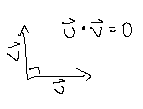
\includegraphics{dot_prod.png} \\
        $\vec{u} \cdot \vec{v} = \magn{\vec{u}} \magn{\vec{v}}\cos \theta$
        \item alg.:
        
        $\vec{u} = \left< u_1, u_2, u_3 \right>$, 
        $\vec{v} = \left< v_1, v_2, v_3 \right>$\\
        $\vec{u} \cdot \vec{v} = \sum u_i v_i$
        \item $\vec{v}\cdot\vec{v} = \magn{\vec{v}}^2$
        \item two vectors are orthogonal aka $\perp$ iff their dot product is $0$
        \item $\displaystyle\cos \theta = \frac{\vec{u} \cdot \vec{v}}{\magn{u}\magn{v}}$ wtf is equation 2.5 "unique over this range" on abt
        \item work $= \vec{F} \cdot \vec{D}$
        \item $\comp$ (scalar projection)
        \begin{align*}
          \comp_{\vec{u}} \vec{v} & = \magn{\vec{v}} \cos \theta \\
          & = \frac{\vec{u} \cdot \vec{v}}{\magn{\vec{u}}}
        \end{align*}
        \item $\proj$ (vector projection)
        \begin{align*}
          \proj_{\vec{u}} \vec{v} &= \comp_{\vec{u}} \vec{v} \cdot \frac{\vec{u}}{\magn{\vec{u}}} \\
          &= \frac{\vec{u}\cdot\vec{v}}{\magn{\vec{u}}^2}\vec{u}
        \end{align*}
      \end{itemize}
    \end{itemize}
  }
  \col{
    \begin{itemize}
      \item Cross Product (3d)
      \begin{itemize}
        \item geom.:
        
        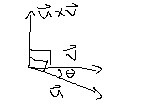
\includegraphics{cross_prod.png}\\
        $\magn{\vec{u}\times\vec{v}} = \magn{\vec{{u}}}\magn{\vec{v}}\sin\theta$
        \item alg.:
        \item $\vec{u} \times \vec{v} = \det\begin{vmatrix}
          \hat{\i} & \hat{\j} & \hat{k}\\
          u_1 & u_2 & u_3 \\
          v_1 & v_2 & v_3
        \end{vmatrix}$
        \item result is $\perp$ to both input vectors, \\
        direction by right hand rule
        \item triple scalar product: \\
        $\vec{u} \cdot (\vec{v}\times\vec{w}) \\ 
        = (\vec{u}\times\vec{v})\cdot\vec{w} \\
        = \det\begin{vmatrix}
          u_1 & u_2 & u_3 \\
          v_1 & v_2 & v_3 \\
          w_1 & w_2 & w_3
        \end{vmatrix}$
        \item if $\vec{u}$ and $\vec{v}$ are the sides of a parallelogram, then its area is $\magn{\vec{u}\times\vec{v}}$
        \item if a parallelepiped has edges $\vec{u}, \vec{v}, \vec{w}$, its volume is the absolute value of its triple scalar product
        \item torque $= \vec{\tau} = \vec{r} \times \vec{F}$
      \end{itemize}
    \end{itemize}
  }
\end{multicols}

\newpage
\begin{multicols}{2}
  \col{
    Lines
    \begin{enumerate}[(1)]
      \item Vector Equation Form
      
      $\vec{r} = \vec{r_0} + t\vec{v}$ \\
      eg $\left<x,y,z\right> = \left<1,2,-5\right> + t\left<3,-4,-1\right>$
      \item Parametric Equation Form
      \begin{align*}
        x &= 1+3t \\
        y &= 2-4t \\
        z &= -5-t 
      \end{align*}
      
      \item Symmetric Equation Form 
      
      solve for $t$
      \[\frac{x-1}{3} = \frac{y-2}{-4} = \frac{z+5}{-1}\]

      \item Edge Case: 0-component
      
      Let a line be defined by the point and vector $(1,-2,6)$ and $\left<3,7,0\right>$. We say the line is:
      \[ \frac{x-1}{3} = \frac{y+2}{7}, z=6 \]
    \end{enumerate}
    \begin{itemize}
      \item point to line distance: use paralleogram area trick
    \end{itemize}

    Planes
    \begin{enumerate}[(1)]
      \item Vector Equation Form
      
      $(\vec{r}-\vec{r_0})\cdot \vec{n} = 0$ \\
      eg $(\left<x,y,z\right>-\left<1,0,1\right>) \cdot \left<1,2,-3\right> = 0$
      \item Scalar Equation, "General" Form
      
      $ax +by +cz +d = 0$
    \end{enumerate}
    \begin{itemize}
      \item point to plane distance: use $\comp_{\vec{u}}\vec{v}$ trick
      \item angle between planes: same as angle between their normal vectors
    \end{itemize}

    Quadric Surfaces
    \begin{itemize}
      \item cylinder: 3d shape consisting of all parallel lines (eg $y=3x^2$)
      \item see \url{quadric_surfaces.pdf}
    \end{itemize}
  }
  \col{
    intentionally blank
  }
\end{multicols}

\newpage
\addsection{Chapter 3: Vector-Valued Functions}
\begin{multicols}{2}
  \col{
    Vector-Valued Function
    $${\vec{r}(t) = \left<f(t), g(t), h(t)\right>}, i < t < j$$

    Unit Circle Parameterization
    
    temp\\

    Limits of VVFs
    \begin{itemize}
      \item pass them into the vec. pretty intuitive
      \item a VVF $\vec{r}(a)$ is cont. at $a$ iff $\displaystyle\lim_{t\rightarrow a}\vec{r}(t) = \vec{r}(a)$ (and both are defined )
    \end{itemize}

    Calc with VVFs
    \begin{itemize}
      \item derivatives are intuitive. use the corresponding dot/cross/scalar in deriving $\vec{u}\cdot\vec{v}$
      \item unit tangent vector is the derivative's unit vector
      \item integrals are intuitive. consider constant vector $C$ instead of scalar constant
    \end{itemize}
  }
  \col{
  }
\end{multicols}

\newpage
\addsection{Appendix} 
\subsection*{matrices, 3x3 determinants}
In depth lesson:
\begin{itemize}
  \item \url{https://www.mathcentre.ac.uk/resources/uploaded/sigma-matrices9-2009-1.pdf}
\end{itemize}

Recall that a elements of a matrix are enumerated $a_{ij}$ where $i$ is column and $j$ is row, both 1-indexed. 
\[\begin{bmatrix}
  a_{11} & a_{12} & a_{13}\\
  a_{21} & a_{22} & a_{23}
\end{bmatrix}\]

Recall that the minor of the matrix element here is the 2 by 2 determinant when you take away the row and column of the element in a 3 by 3 matrix.  Picking an arbitrary row (or even column), with $a_{ij}$ being an element and $M_{ij}$ being a minor, a 3 by 3 determinant is calculated by 
\[ \sum_{j=1}^{3} (-1)^{i+j} a_{ij} M_{ij} \]
In the figure \texttt{media/3x3determinant.png}, $(-1)^{i+j}$ is in green, $a_{ij}$ in orange, and $M_{ij}$ in blue.

\subsection*{cross/dot products}
\begin{itemize}
  \item see:
  \begin{itemize}
    \item \url{media/cross_prod_area_ex.png}
    \item \url{media/scalar_projection_composition_ex.png}
    \item \url{media/scalar_triple_prod_parallelepiped_ex.png}
  \end{itemize}
\end{itemize}






%%%%%%%%%%%%%%%%%%%%%%%%%%%%
%% End of document body   %%
%%%%%%%%%%%%%%%%%%%%%%%%%%%%
\end{document}
